\section{Advent Nopele Sihite}

\subsection{Teori}
	
	\subsubsection{Jelaskan kenapa kata-kata harus di lakukan vektorisasi. dilengkapi dengan ilustrasi atau gambar.}
	\hfill\\
	Algoritma machine learning perlu mengubah teks menjadi angka terlebih dahulu agar dapat dibaca oleh komputer, karena komputer hanya mengerti bahasa biner.Vektorisasi membantu mengubah teks kedalam bentuk vektor yang dapat dimengerti oleh komputer. 
	
	\begin{figure}[H]
		\begin{center}
		 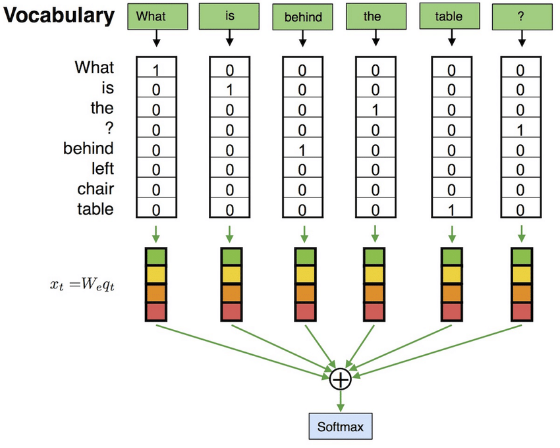
\includegraphics[width=10cm]{figures/1174076/figures5/teori1.png}
		 \caption{Soal 1}	
		\end{center}
	\end{figure}

	\subsubsection{Jelaskan mengapa dimensi dari vektor dataset google bisa sampai 300.dilengkapi dengan ilustrasi atau gambar.}
	\hfill\\
	Karena google memiliki setidaknya 3 Milyar kata dan kalimat yang unik(berbeda-beda) dalam satu dataset.
	
	\begin{figure}[H]
		\begin{center}
		 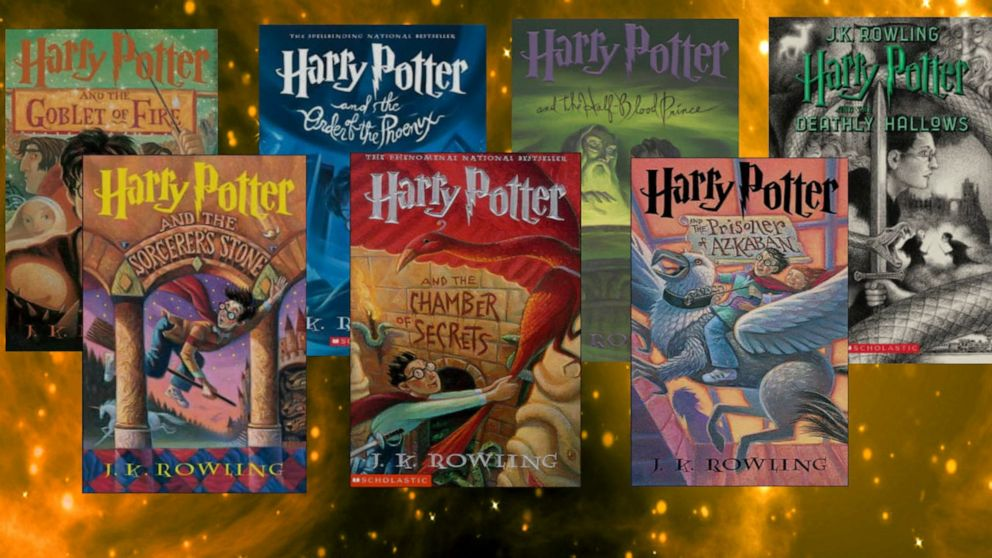
\includegraphics[width=10cm]{figures/1174076/figures5/teori2.png}
		 \caption{Soal 2}	
		\end{center}
	\end{figure}
	
	Untuk ilustrasinya, misalkan kita memiliki sebuah buku dengan tebal 1000 , dimana bukunya dibagi menjadi dua Chapter. Kemudian kita akan menggabungkan kata dari setiap Chapter tersebut. Maka akan didapatkan irisan yang akan berjumlah lebih dari 200. dikarenakan banyak kata yang berbeda beda.


	\subsubsection{Jelaskan konsep vektorisasi untuk kata.dilengkapi dengan ilustrasi atau gambar.}
	\hfill\\
	Konsepnya yaitu kata atau teks akan dihapuskan noisy datanya atau dihapus data yang tidak terpakai,seperti tag html jika ada,titik,koma,dll. Kemudian tokenization artinya kita akan mengelompokan kalimat menjadi token atua membagi kata kata menjadi potingan kecil. Baru setelah itu dilakukan normalisasi untuk mengubah datanya menjadi angka.

	\begin{figure}[H]
		\begin{center}
		 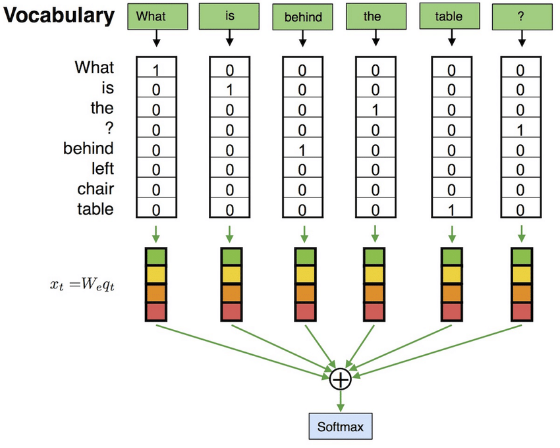
\includegraphics[width=10cm]{figures/1174076/figures5/teori1.png}
		 \caption{Soal 3}	
		\end{center}
	\end{figure}
	
	\subsubsection{Jelaskan konsep vektorisasi untuk dokumen.dilengkapi dengan ilustrasi atau gambar.}
	\hfill\\
	Pada dokumen akan diprediksi seberapa sering muncul kata dalam 2 kalimat atau 2 paragraf. Dengan Doc2Vec bisa diprediksi.Doc2Vec merupakan model yang dapat mengitung kemiripan atau kecocokan pada sebuah kalimat.
	
	\begin{figure}[H]
		\begin{center}
		 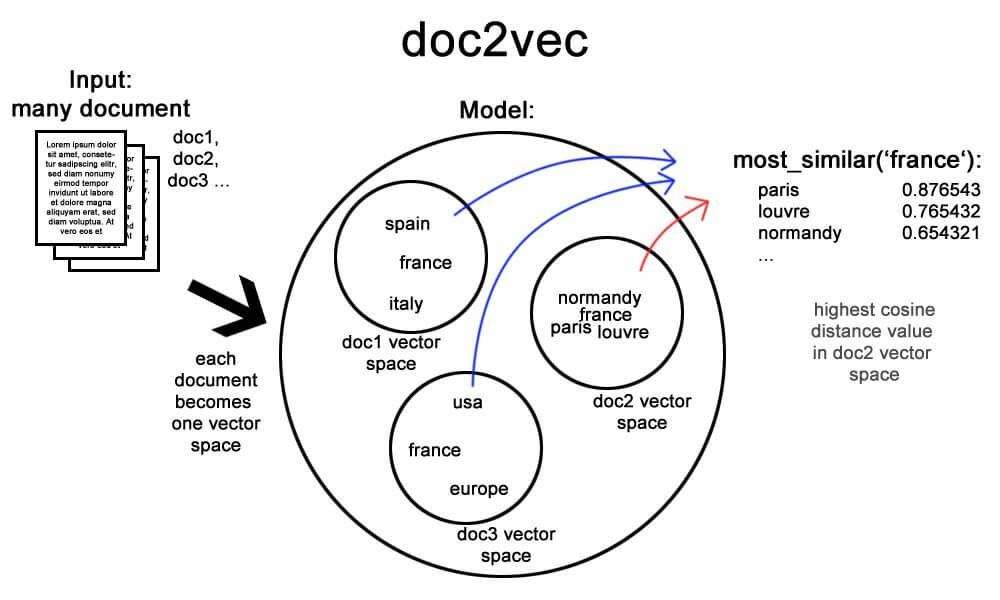
\includegraphics[width=10cm]{figures/1174076/figures5/teori4.png}
		 \caption{Soal 4}	
		\end{center}
	\end{figure}
	
	\subsubsection{Jelaskan apa mean dan standar deviasi,dilengkapi dengan ilustrasi atau gambar.} 
	\hfill\\
	Mean adalah rata-rata nilai dari sekumpulan data.Sedangkan standar deviasi adalah nilai statistik yang dimanfaatkan untuk menentukan bagaimana sebaran data dalam sampel, serta seberapa dekat titik data individu ke mean atau rata-rata nilai sampel. Ini berguna dalam membandingkan set data yang mungkin memiliki mean yang sama tetapi rentang yang berbeda.
	
	\begin{figure}[H]
		\begin{center}
		 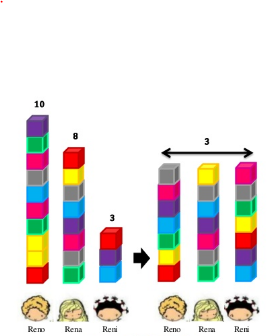
\includegraphics[width=10cm]{figures/1174076/figures5/teori5.png}
		 \caption{Soal 5}	
		\end{center}
	\end{figure}
	
	\subsubsection{Jelaskan apa itu skip-gram,dilengkapi dengan ilustrasi atau gambar.}
	\hfill\\
	Secara Arsitektur Skip-Gram menggunakan current word (sebagai input) untuk memprediksi konteks (sebagai target) disekitarnya, dimana Skip-Gram akan mempelajari distribusi probabilitas dari kata-kata didalam konteks dengan windows yang telah di tentukan.
	
	\begin{figure}[H]
		\begin{center}
		 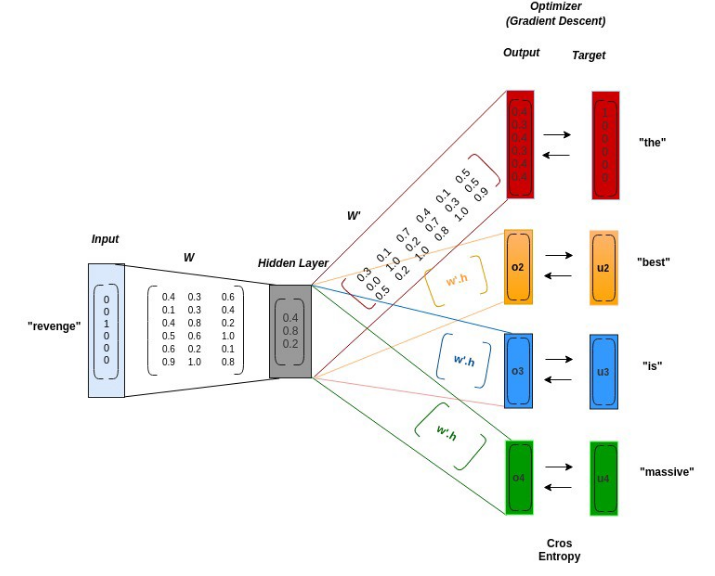
\includegraphics[width=10cm]{figures/1174076/figures5/teori6.png}
		 \caption{Soal 6}	
		\end{center}
	\end{figure}
		
\subsection{Praktek}

	\subsubsection{Cobalah dataset google, dan jelaskan vektor dari kata love, faith, fall, sick, clear, shine, bag, car, wash, motor, cycle dan cobalah untuk melakukan perbandingansimilirati dari masing-masing kata tersebut. jelaskan arti dari outputan similaritas dan setiap baris kode yang dibuat(harus beda dengan teman sekelas). (Nilai 5 untuk setiap perbandingan, disini ada 5 perbandingan similaritas)}\hfill\\
	
	\subsubsection{jelaskan dengan kata dan ilustrasi fungsi dari extract words dan PermuteSentences (harus beda dengan teman sekelas)
}\hfill\\
	
	\subsubsection{ Jelaskan fungsi dari librari gensim TaggedDocument dan Doc2Vec disertai praktek pemakaiannya. Tunjukkan keluarannya dari komputer sendiri dan artikan
maksud setiap luaran yang didapatkan.}\hfill\\
	
	\subsubsection{Jelaskan dengan kata dan praktek cara menambahkan data training dari file
yang dimasukkan kepada variabel dalam rangka melatih model doc2vac. Tunjukkan keluarannya dari komputer sendiri dan artikan maksud setiap luaran
yang didapatkan.}\hfill\\
	
	\subsubsection{Jelaskan dengan kata dan praktek kenapa harus dilakukan pengocokan dan
pembersihan data. Tunjukkan keluarannya dari komputer sendiri dan artikan
maksud setiap luaran yang didapatkan.}\hfill\\

	\subsubsection{Jelaskan dengan kata dan praktek kenapa model harus di save dan kenapa
temporari training harus dihapus.Tunjukkan keluarannya dari komputer sendiri
dan artikan maksud setiap luaran yang didapatkan.
}\hfill\\
	
	\subsubsection{jalankan dengan kta dan praktek maksud dari infer code. Tunjukkan keluarannya dari komputer sendiri dan artikan maksud setiap luaran yang didapatkan.}\hfill\\
	
	\subsubsection{Jelaskan dengan praktek dan kata maksud dari cosine similarity. Tunjukkan
keluarannya dari komputer sendiri dan artikan maksud setiap luaran yang didapatkan.}\hfill\\

	\subsubsection{Jelaskan dengan praktek score dari cross validation masing-masing metode.
Tunjukkan keluarannya dari komputer sendiri dan artikan maksud setiap luaran yang didapatkan}\hfill\\
	
\subsection{Penangan Error}
	
	\subsubsection{Screenshoots Error}\hfill\\
	
	\subsubsection{Tuliskan kode eror dan jenis errornya}\hfill\\
	 
	\subsubsection{Solusi pemecahan masalah error tersebut}\hfill\\
	
	
\subsection{Link Youtube}
	
	\subsubsection{}\hfill\\

	